\chapter{\label{ch:4}MWC modelling} 

\graphicspath{{figures/ch4/}}

\minitoc

\section{Modelling nucleotide regulation of the K\ATP{} channel}

The complex regulation of K\ATP{} channel activity by nucleotides and phosphoinositides has led to a wide range of scientists seeking to unify the constellation of structural and functional studies into one mechanistic framework, which is capable of explaining each aspect of channel regulation.
The importance of K\ATP{} channels in regulating insulin secretion, responding to cardiac stress, and protecting against seizures is one driving force behind the search for a model \cite{proks_modeling_2009}.
Another aim is more holistic; hoping that increasing our understanding of how the K\ATP{} channel is regulated by the interplay of its ligands may shed light on other ion channels or proteins \cite{garfinkel_modeling_2017}.
In any case, the primary goal of constructing a mathematical model of the K\ATP{} channel is to explain as much of the diversity of channel function as possible, while keeping the model as simple and biologically relevant as possible; a balancing act between completeness and complexity.

Previous attempts at modelling K\ATP{} channel regulation have primarily focused on nucleotide inhibition \cite{trapp_molecular_1998, enkvetchakul_kinetic_2000, markworth_atp4-_2000, ribalet_regulation_2000, enkvetchakul_atp_2001-1, drain_concerted_2004, proks_gating_2005, li_ligand-dependent_2005, ribalet_atp-sensitive_2006-1, craig_how_2008-1}, due to the relative ease of isolating the effects of nucleotide inhibition.
There have been fewer attempts at incorporating activation by Mg-nucleotides \cite{ribalet_regulation_2000, proks_activation_2010-1, vedovato_nucleotide-binding_2015}.
The difficulty in quantifying phosphinositide regulation of the K\ATP{} channel means that in most cases where it is considered, it is implicitly included as a component of the intrinisc gating of the channel, rather than explicitly described \cite{baukrowitz_pip2_1998, fan_phosphoinositides_1999, enkvetchakul_kinetic_2000}, although there are some exceptions \cite{ribalet_regulation_2000, enkvetchakul_atp_2001-1, enkvetchakul_gating_2003}.

What does a model of ion channel function look like?
Broadly, a model attempts to categorise discrete conformational states of the channel, and describe the transitions between those states.
In the simplest case, an ion channel can be described as fluctuating between an open state and a closed state (Figure \ref{ch4fig:simple_model_diagram}).
As these states exist in equilibrium, they can be described by an equilbrium constant ($L$) which is composed of the rate constant for the opening transition ($k_O$) divided by the rate constant for the closing transition ($k_C$).

\begin{figure}[h]
	\centering
	\begin{subfigure}[t]{0.45\textwidth}
		\caption{}\label{ch4fig:simple_diag_1}
		\centering
		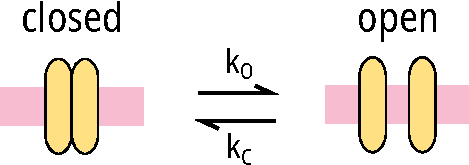
\includegraphics[width=\textwidth]{model_introduction_diagrams.pdf}
	\end{subfigure}
	\hfill
	\begin{subfigure}[t]{0.45\textwidth}
		\caption{}\label{ch4fig:simple_diag_2}
		\centering
		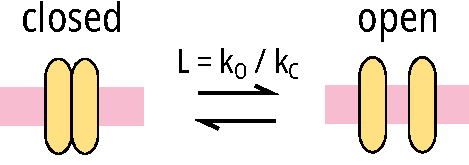
\includegraphics[width=\textwidth]{model_introduction_diagrams_2.pdf}
	\end{subfigure}
	\caption[Simple ion channel model]{
	The transition between two states, open and closed, can be described either by two kinetic constants (\subref{ch4fig:simple_diag_1}) for the opening ($k_O$) and closing ($k_C$), or by an equilibrium constant $L$ (\subref{ch4fig:simple_diag_2}), which is equal to $\frac{k_O}{k_C}$.
	}\label{ch4fig:simple_model_diagram}
\end{figure}

To relate this to empirical measurements of ion channel function, $L$ is equivalent to the $P_O$ of this two-state channel.
Alternatively, in this simple two-state channel, $k_O$ and $k_C$ can be calculated directly by measuring the lifetimes of the closed and open states respectively from single-channel recordings \cite{reinhold_penner_auth_single-channel_1995, sivilotti_praise_2016}.
Of course, real ion channels are more complicated and two states are not sufficient to describe the complexity of the ligand regulation of K\ATP{} channels, which visit a multitude of conformational states.
As our understanding of the channel grows, the more complex a model needs to be to fully account for all observed aspects of function (Figure \ref{ch4fig:standards}).

\begin{figure}[h]
	\centering
	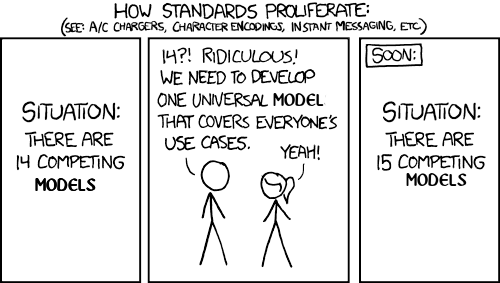
\includegraphics[width=0.7\textwidth]{xkcd_standards.png}
	\caption{
	Adapted from Randall Munroe (https://xkcd.com/927/).
	}\label{ch4fig:standards}
\end{figure}

\subsection{Restricting the subset of possible models}


\subsection{Determining open probability}
Noise analysis - you can get a correct answer the wrong way (Puljung).

Measuring the open probability of an ion channel is most accurately accomplished by single-channel electrophysiological recordings, which allows direct measurement of the time a channel spends in an open state.
This approach does not allow for the determination of the open probability of a population of channels great than 2/3 at a time, as it becomes increasingly difficult to separate the openings of different channels in the population.
Thus it would not be possible to determine single channel open probability simultaneously with nucleotide binding, as the fluorescence signal from a small number of channels would be impossible to resolve.

Another approach is noise analysis of currents from large populations of channels.
The 'noise' in noise analysis refers to current fluctuations which occur when recording from a population of ion channels due to the stochastic channel gating of individual channels.
If there are a constant number of channels ($N$) which are gated independently from each other and share a homogenous open probability ($P_O$) and a single open conductance level ($i$), the observed macroscopic current level $I$ can be described by equation \ref{eq:inpo}:
\begin{equation}\label{eq:inpo}
	I = iNP_O
\end{equation}
and the observed variance of the macroscopic current can be described by the variance of the binomial distribution, equation \ref{eq:bin_1}:
\begin{equation}\label{eq:bin_1}
	\sigma^2 = NP_O \cdot (1 - P_O) \cdot i^2
\end{equation}
where the single channel current is essentially a scaling factor.
If we assume that in a given recording $N$ and $i$ remain constant, and it is $P_O$ which changes in response to any given stimuli, then we can combine equations \ref{eq:inpo} and \ref{eq:bin_1} to yield equation \ref{eq:bin_2}:
\begin{equation}\label{eq:bin_2}
	\sigma^2 = iI - \frac{1}{N} \cdot I^2
\end{equation}
This equation yields a parabola from $I = 0$ to $I = Ni$.
Intuitively, there can be no variance when $P_O$ is exactly 0 or 1, as there will be no opening or closing events which can give rise to current fluctuations.
Once $i$ and $N$ have been determined for a given experiment, the observed current magnitude $I$ can be converted into the $P_O$ for the population of channels by rearranging equation \ref{eq:inpo} as follows:
\begin{equation}\label{eq:poin}
	P_O = \frac{I}{iN}
\end{equation}

Equation \ref{eq:bin_2} can be fit to experimental data by calculating the variance of observed current at different current magnitudes.
This calculation is not exactly trivial, and has been accomplished a number of different ways for different purposes.
For channels with fast inactivation such as the Na\textsubscript{V} family, non-stationary noise analysis involves repeating a stimulus multiple times and measuring variance as the squared sum of deviations from the mean of the current magnitude calculated at the same time point across multiple stimuli, referred to in the literature as an 'isochrone'.
For channels which do not inactivate, stationary noise analysis is possible, and variance can be measured as the squared sum of deviations from the mean current magnitude over a period of time for which $I$ is 'stationary'(Figure \ref{ch4fig:noise_example_1}, \ref{ch4fig:noise_example_2}, \ref{ch4fig:noise_example_3}).

Stationary noise analysis has been described for K\ATP{} channels before by a number of different researchers (Shyng, Paolo, Peter).
Unfortunately, in most of the published research the exact procedure for extracting the parameters in equation \ref{eq:bin_1} is described in the methods section, but the quality of the fits and the value of the fitted parameters besides the final calculated $P_O$ is not discussed.
A notable exception to this rule is (Paolo), in which two findings are discussed.
Firstly, fitting equation \ref{eq:bin_2} to the mean and variance of \SI{200}{\milli\second} sections of macroscopic currents from wild-type Kir6.2+SUR2A resulted in a systematic underestimation of the single channel current $i$.
From single channel experiments, the single channel current was determined to be \SI{4}{\pico\ampere}, while the value obtained from fitting macroscopic currents was only \SI{2}{\pico\ampere}.
In the case of WT-GFP+SUR1, we see a similar understimation of single channel current (Figure \ref{ch4fig:noise_example_fits_1}, \ref{ch4fig:noise_example_fits_2}, \ref{ch4fig:noise_example_fits_3}), with fits yielding estimates of \SIrange{1.66}{2.64}{\pico\ampere}, while measured single channel currents are at least \SI{4}{\pico\ampere}.
This underestimate of $i$ is most likely due to an underestimate of channel current variance as $P_O$ increases, which could be due to two main reasons.

Firstly, the process of filtering and digitising channel currents can lead to underestimates of variance depending on the relationship between the open time of the measured channel and the cut-off frequency of the filter used.
It is unlikely that this phenomenon is responsible for our findings, as the K\ATP{} mean open time duration is close to \SI{1}{\milli\second} and filtering at \SI{5}{\kilo\hertz} would lead to less than a \SI{5}{\percent} underestimation of $i$.
Even if the mean open time of WT-GFP+SUR1 was closer to \SI{0.1}{\milli\second}, we would expect a \SI{20}{\percent} reduction rather than the \SI{50}{\percent} we actually observe.
Empirically, we can use the frequency power spectrum of our measured current fluctuations to determine whether there may be high frequency channel openings we are missing (Figure \ref{ch4fig:spectra_converge}).
For WT-GFP+SUR1, we observe that at frequencies approaching our filter cut-off at \SI{5}{\kilo\hertz} there is very little observed amplitude in active channels when compared to fully inhibited channels, suggesting we are not missing high frequency current fluctuations.

\begin{figure}[h]
	\centering
	\begin{subfigure}[t]{0.3\textwidth}
		\caption{}\label{ch4fig:noise_example_1}
		\centering
		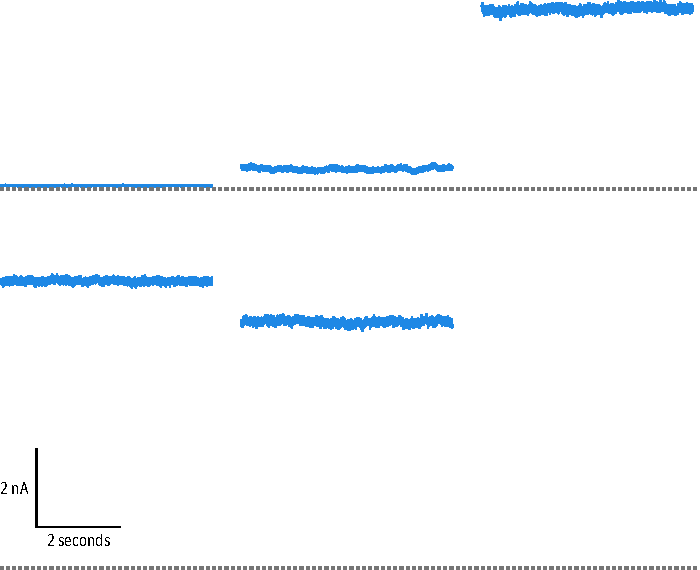
\includegraphics[width=\textwidth]{noise_example_1.pdf}
	\end{subfigure}
	\hfill
	\begin{subfigure}[t]{0.3\textwidth}
		\caption{}\label{ch4fig:noise_example_2}
		\centering
		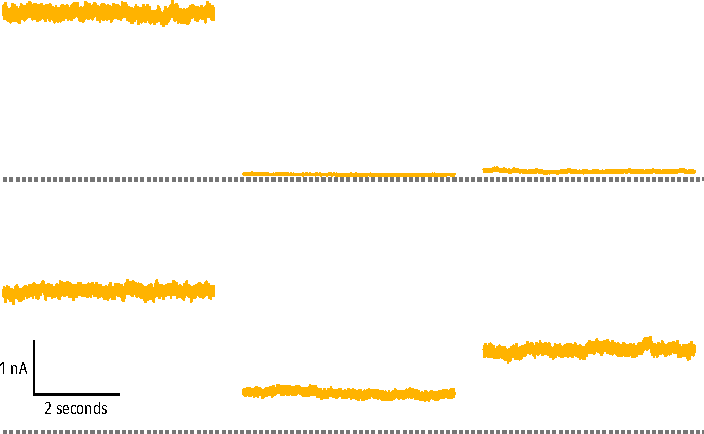
\includegraphics[width=\textwidth]{noise_example_2.pdf}
	\end{subfigure}
	\hfill
	\begin{subfigure}[t]{0.3\textwidth}
		\caption{}\label{ch4fig:noise_example_3}
		\centering
		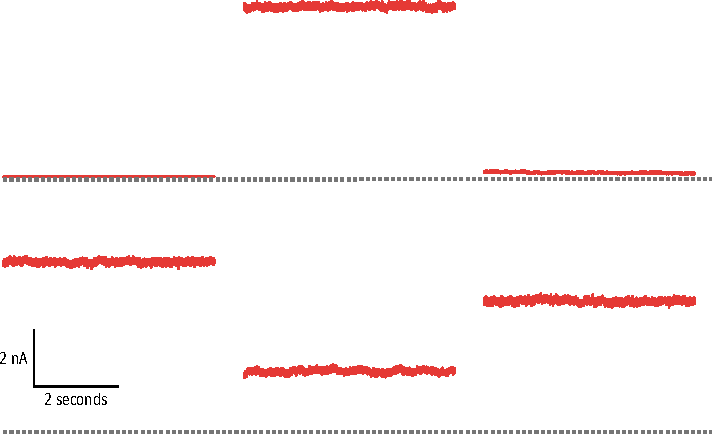
\includegraphics[width=\textwidth]{noise_example_3.pdf}
	\end{subfigure}
	\vfill
	\begin{subfigure}[t]{0.3\textwidth}
		\caption{}\label{ch4fig:noise_example_fits_1}
		\centering
		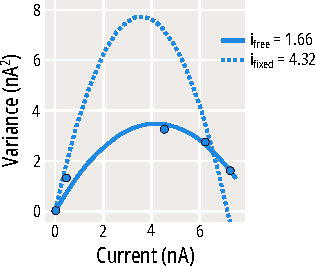
\includegraphics[width=\textwidth]{noise_example_fits_1.pdf}
	\end{subfigure}
	\hfill
	\begin{subfigure}[t]{0.3\textwidth}
		\caption{}\label{ch4fig:noise_example_fits_2}
		\centering
		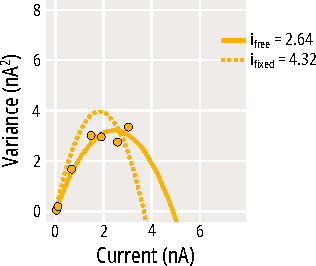
\includegraphics[width=\textwidth]{noise_example_fits_2.pdf}
	\end{subfigure}
	\hfill
	\begin{subfigure}[t]{0.3\textwidth}
		\caption{}\label{ch4fig:noise_example_fits_3}
		\centering
		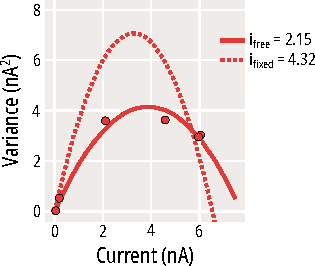
\includegraphics[width=\textwidth]{noise_example_fits_3.pdf}
	\end{subfigure}
	\vfill
	\begin{subfigure}[t]{0.5\textwidth}
		\caption{}\label{ch4fig:spectra_converge}
		\centering
		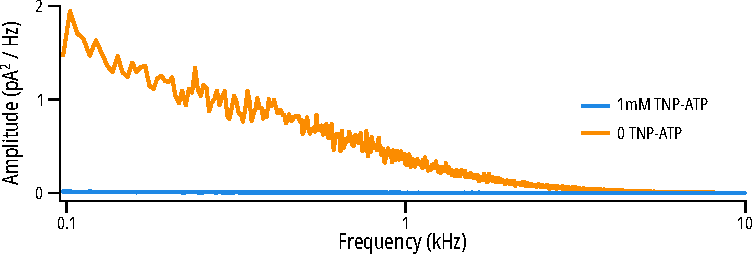
\includegraphics[width=\textwidth]{spectra_converge.pdf}
	\end{subfigure}
	\caption[Systematic underestimation of single channel currents]{
	\subref{ch4fig:noise_example_1},\subref{ch4fig:noise_example_2},\subref{ch4fig:noise_example_3} 5 second extracts from three separate recordings of WT-GFP+SUR1 currents.
	Extracts from different recordings are coloured differently.
	The zero current level determined by barium is indicated as a dashed line.
	\subref{ch4fig:noise_example_fits_1}, \subref{ch4fig:noise_example_fits_2}, \subref{ch4fig:noise_example_fits_3} Plots of the mean current and variance for each of the extracts in the panel above.
	Fits to equation x are shown as a solid line when $i$ is allowed to vary freely, and as a dashed line when $i$ is fixed to \SI{4.32}{\pico\ampere}.
	The fitted value for $i$ is shown for each recording separately.
	\subref{ch4fig:spectra_converge} Averaged power spectra for the three recordings analysed.
	The blue line is the power spectra when channels are fully inhibited and represents the background, while the orange line is the power spectra when channels are most active.
	The high frequency components of the current fluctuations are attenuated to near background levels above \SIrange{2}{3}{\kilo\hertz}.
	}\label{ch4fig:noise_manual}
\end{figure}

Secondly, an underestimation of $i$ could occur due to violations in the underlying assumptions of the binomial distribution.
The first two assumptions are that $N$ and $i$ are constant throughout a recording.
We know that $i$ does not change on nucleotide inhibition of K\ATP{} channels, noris it affected by PIP\textsubscript{2} and rundown.
Additionally, in excised patches it is improbable that there will be any change in $N$ during the course of a recording.
The third assumption is that the channels in a patch share a homogenous $P_O$, which exhibits graded changes in response to stimuli (in our case, application of nucleotide).
This assumption is far harder to justify for our experimental condition, in which channel rundown due to loss of PIP\textsubscript{2} results in a complicated mixture of channel populations with different $P_O$s.

An extreme case in which channels transition between two states, one where $0 < P_O < 1$ and one where $P_O \approx 0$ can be approximated by equation \ref{eq:bin_1}, with a channel transitioning to the $P_O \approx 0$ state essentially considered to be no longer available to open, thus reducing $N$.
Thus, fitting the observed current-variance data with \ref{eq:bin_1} would yield a straight line where the slope of the line is equal to $i \cdot (1 - P_O)$.
This formulation of equation \ref{eq:bin_1} has been used successfully in the analysis of currents from CRAC channels, VSOA channels, and in the analysis of a specific cardiac K\ATP{} channel mutation.
Unfortunately, in our case channel rundown does not render the K\ATP{} channel completely unable to open, with fully rundown channels displaying single channel open probabilities in the range of \numrange{0.05}{0.25}.
Instead of each current measurement being a draw from a single binomial distribution, we are instead drawing from a mixture of binomial distributions with different $P_O$s.
We can demonstrate how this leads to an underestimation of $i$ by simulating a simple case where there are two populations of channels, $a$ and $b$, one with a tenfold lower $P_O$ than the other.

\begin{equation}\label{eq:bibi_sim}
\begin{split}
	N_a + N_b &= 1000 \\
	0 < P_{O_{a}} &< 1 \\
	P_{O_{b}} &= \frac{P_{O_{a}}}{10}
\end{split}
\end{equation}

\begin{figure}[h]
	\centering
	\begin{subfigure}[t]{0.3\textwidth}
		\caption{}\label{ch4fig:simulated_noise_1}
		\centering
		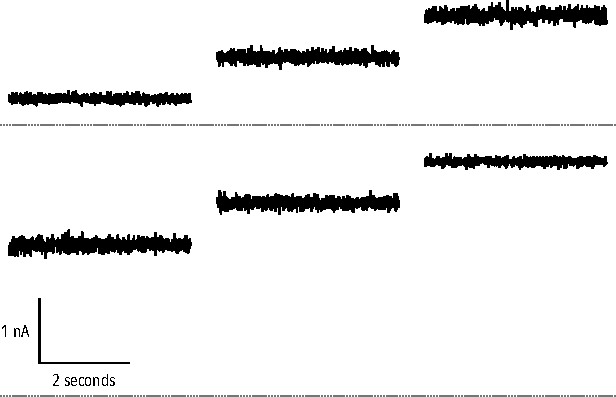
\includegraphics[width=\textwidth]{simulated_noise_1.pdf}
	\end{subfigure}
	\hfill
	\begin{subfigure}[t]{0.3\textwidth}
		\caption{}\label{ch4fig:simulated_noise_2}
		\centering
		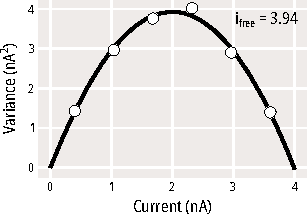
\includegraphics[width=\textwidth]{simulated_noise_2.pdf}
	\end{subfigure}
	\hfill
	\begin{subfigure}[t]{0.3\textwidth}
		\caption{}\label{ch4fig:simulated_noise_3}
		\centering
		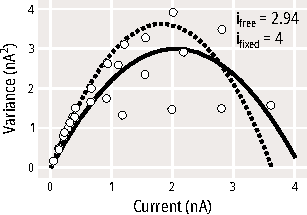
\includegraphics[width=\textwidth]{simulated_noise_3.pdf}
	\end{subfigure}
	\caption[Simulated multibinomial currents]{
	}\label{ch4fig:noise_sim}
\end{figure}

\begin{figure}[h]
	\centering
	\begin{subfigure}[t]{0.9\textwidth}
		\caption{}\label{ch4fig:noise_fits_1}
		\centering
		\includegraphics[width=\textwidth]{noise_fits_1.pdf}
	\end{subfigure}
	\vfill
	\begin{subfigure}[t]{0.9\textwidth}
		\caption{}\label{ch4fig:noise_fits_2}
		\centering
		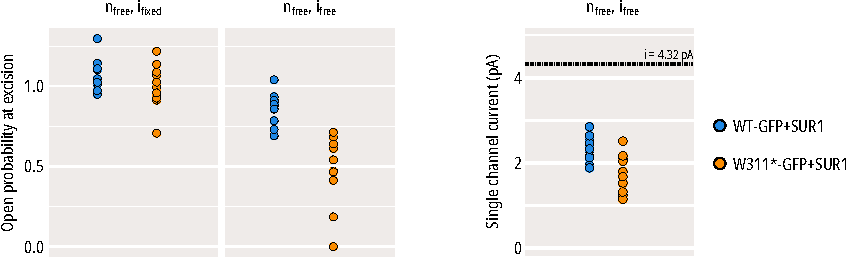
\includegraphics[width=\textwidth]{noise_fits_2.pdf}
	\end{subfigure}
	\caption[Estimating open probability from stationary noise analysis]{
	\subref{ch4fig:noise_fits_1} Plots of the mean current and variance for 1 second extracts from recordings of WT-GFP+SUR1 (blue) or W311*-GFP+SUR1 (orange).
	Fits to equation x are shown as a solid line when $i$ is allowed to vary freely, and as a dashed line when $i$ is fixed to \SI{4.32}{\pico\ampere}.
	The straight, finer dashed lines are fits to equation y only using the linear portion of the data, which are shown as solid filled points outlined in black.
	\subref{ch4fig:noise_fits_2} Parameter estimates from fits in \subref{ch4fig:noise_fits_1} are shown as separate points for each experiment.
	For fits to equation x, open probability is calculated from the intial current on patch excision.
	To visualise the spread, normal distributions are plotted alongside the point estimates, limited to $0 < x < 1$.
	}\label{ch4fig:all_noise_fits}
\end{figure}

\section{Implementing an MWC model}

\subsection{A simple case}

The simplest case of an allosteric MWC model for an ion channel is shown as Scheme I in Figure \ref{ch4fig:mwc_model_diagrams}.
This simple case assumes a channel composed of a single monomer with a single binding site for ligand $A$.
The channel is restricted to two states, open and closed.
These two states exist in an equilibrium described by L, which is equivalent to $\frac{[open]}{[closed]}$.
Ligand $A$ binds to the protein with a microscopic affinity constant $K_A$.
The ligand $A$ differentially stabilises the open and closed states by a constant $D$.
When $D$ is unity, the ligand $A$ binds equally to both states and so does not influence the conformational changes of the channel.
When $D>1$, the ligand $A$ preferentially stabilises the open state, while when $D<1$ the ligand instead preferentially stabilises the closed state.

\begin{figure}[h]
	\centering
	\begin{subfigure}[t]{0.9\textwidth}
		\caption{}\label{ch4fig:mwc_model_diagrams}
		\centering
		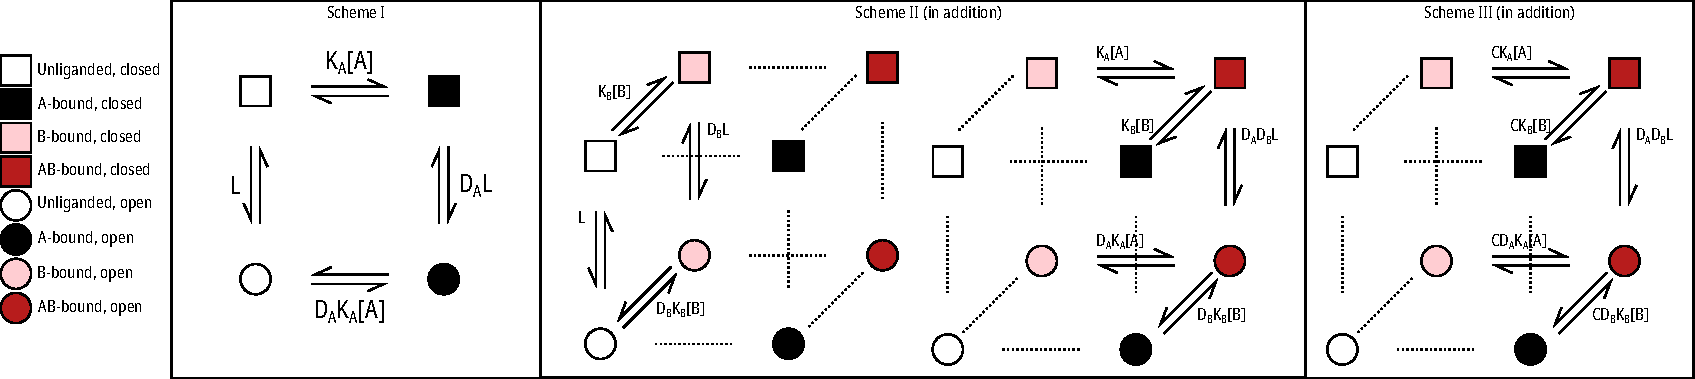
\includegraphics[width=\textwidth]{mwc_model_diagrams.pdf}
	\end{subfigure}
	\vfill
	\begin{subfigure}[t]{0.3\textwidth}
		\caption{}\label{ch4fig:mwc_scheme_1_fits}
		\centering
		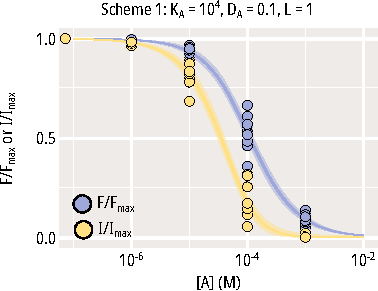
\includegraphics[width=\textwidth]{mwc_scheme_1_fits.pdf}
	\end{subfigure}
	\hfill
	\begin{subfigure}[t]{0.3\textwidth}
		\caption{}\label{ch4fig:mwc_scheme_2_fits}
		\centering
		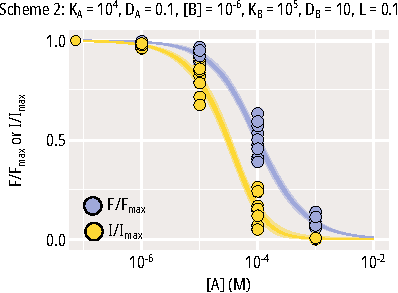
\includegraphics[width=\textwidth]{mwc_scheme_2_fits.pdf}
	\end{subfigure}
	\hfill
	\begin{subfigure}[t]{0.3\textwidth}
		\caption{}\label{ch4fig:mwc_scheme_3_fits}
		\centering
		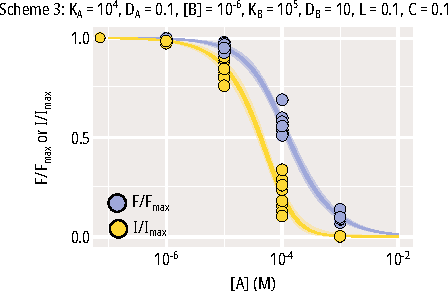
\includegraphics[width=\textwidth]{mwc_scheme_3_fits.pdf}
	\end{subfigure}
	\vfill
	\begin{subfigure}[t]{0.9\textwidth}
		\caption{}\label{ch4fig:mwc_params_1}
		\centering
		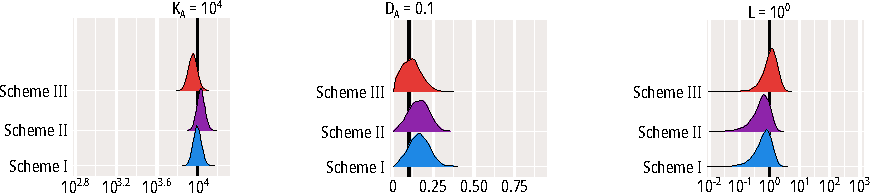
\includegraphics[width=\textwidth]{mwc_scheme_param_fits.pdf}
	\end{subfigure}
	\caption[Generating data from MWC model schemes]{
	\subref{ch4fig:mwc_model_diagrams} Equilibrium diagrams for the three MWC schemes considered.
	For each scheme, only the parameters newly relevant for that scheme are shown explicitly.
	\subref{ch4fig:mwc_scheme_1_fits}, \subref{ch4fig:mwc_scheme_2_fits}, \subref{ch4fig:mwc_scheme_3_fits} Data generated from Scheme I (\subref{ch4fig:mwc_scheme_1_fits}), Scheme II (\subref{ch4fig:mwc_scheme_2_fits}) or Scheme III (\subref{ch4fig:mwc_scheme_3_fits}) all fit to Scheme I.
	The input parameters are shown above each panel.
	$L$ differs between \subref{ch4fig:mwc_scheme_1_fits} and \subref{ch4fig:mwc_scheme_2_fits}, \subref{ch4fig:mwc_scheme_3_fits} due to the introduction of a resting PIP\textsubscript{2} concentration, which in Scheme I is implicitly incorporated into $L$.
	\subref{ch4fig:mwc_params_1} Parameter estimates for the Scheme I model fit to the data generated by all three schemes.
	The input parameter value is marked as a black vertical line for each panel.
	}\label{ch4fig:mwc_models}
\end{figure}

\subsection{The role of PIP\textsubscript{2}}

If we consider introducing a second ligand B which binds to a distinct site on the same monomer and does not directly interact with ligand A, we introduce the states shown in Scheme II of Figure \ref{ch4fig:mwc_model_diagrams}.
Each ligand has its own microscopic association constant ($K_A$ or $K_B$) and its own preference for the open or closed states ($D_A$ or $D_B$).
Importantly, there is no interaction term between ligand $A$ and ligand $B$; the only way the binding of the ligands can impact each other is through effects on $L$.
Scheme II is therefore a restricted form of scheme III, which explicity introduces a term for local interaction ($C$) between binding sites for ligands $A$ and $B$ on the same monomer.
When $C$ is unity, Scheme III becomes Scheme II.
When $C<1$, binding of one ligand reduces the ability of the other ligand to bind on the same monomer.
When $C>1$, binding of one ligand enhances the ability of the other ligand to bind on the same monomer.

To study nucleotide binding to Kir6.2, I have used Scheme I (expanded to incorporate four identical monomers) as an approximation of the K\ATP{} channel, with ligand $A$ representing nucleotides.
To determine whether this approximation is appropriate, I generated data using each of the three schemes as the underlying model of channel function and then fit the generated observations to Scheme I (Figure \ref{ch4fig:mwc_scheme_1_fits}, \ref{ch4fig:mwc_scheme_2_fits}, \ref{ch4fig:mwc_scheme_3_fits}).
Ten individual sets of observations were generated using the inputs shown above each figure panel as the centre of a lognormal distribution with a standard deviation of 0.25.
These observations were then fit to Scheme I (as done previously throughout the thesis) and the values of the three free parameters ($K_A$, $D_A$ and $L$) were estimated (Figure \ref{ch4fig:mwc_params_1}).

\begin{figure}[h]
	\centering
	\begin{subfigure}[t]{0.3\textwidth}
		\caption{}\label{ch4fig:scheme_1_ka_shift}
		\centering
		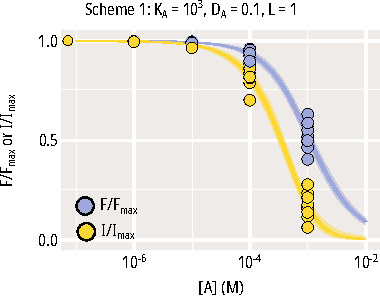
\includegraphics[width=\textwidth]{mwc_scheme_1_ka_shift.pdf}
	\end{subfigure}
	\hfill
	\begin{subfigure}[t]{0.3\textwidth}
		\caption{}\label{ch4fig:scheme_1_da_shift}
		\centering
		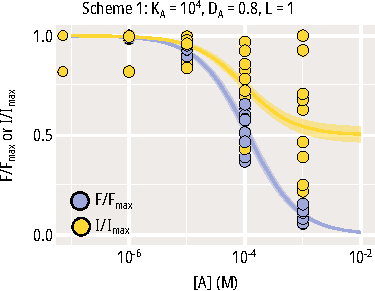
\includegraphics[width=\textwidth]{mwc_scheme_1_da_shift.pdf}
	\end{subfigure}
	\hfill
	\begin{subfigure}[t]{0.3\textwidth}
		\caption{}\label{ch4fig:scheme_1_l_shift}
		\centering
		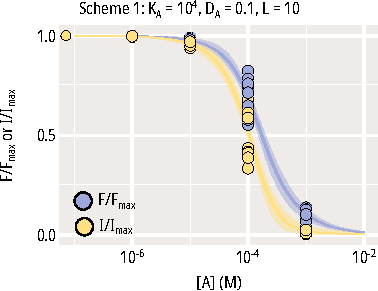
\includegraphics[width=\textwidth]{mwc_scheme_1_l_shift.pdf}
	\end{subfigure}
	\vfill
	\begin{subfigure}[t]{0.9\textwidth}
		\caption{}\label{ch4fig:mwc_params_2}
		\centering
		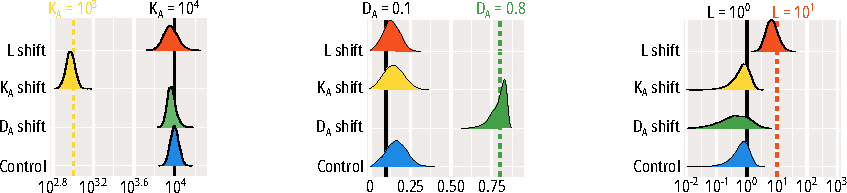
\includegraphics[width=\textwidth]{mwc_scheme_param_fits_2.pdf}
	\end{subfigure}
	\caption[Parameter retrieval from MWC models]{
	\subref{ch4fig:scheme_1_ka_shift}, \subref{ch4fig:scheme_1_da_shift}, \subref{ch4fig:scheme_1_l_shift} Data generated from Scheme I with \subref{ch4fig:scheme_1_ka_shift} $K_A$ shifted from $10^4$ to $10^3$, \subref{ch4fig:scheme_1_da_shift} $D_A$ shifted from $0.1$ to $0.8$, or \subref{ch4fig:scheme_1_l_shift} $L$ shifted from $1$ to $10$.
	\subref{ch4fig:mwc_params_} Parameter estimates from each of the model fits.
	In each case, the modified parameter is retrieved accurately and no other parameters are affected.
	}\label{ch4fig:scheme_1_shifts}
\end{figure}

We know that Scheme I is only an approximation of nucleotide binding as it does not explicitly include PIP\textsubscript{2}.
The question is, if the underlying data generating model is Scheme II which explicitly includes a second ligand, are we still able to extract meaningful parameter estimates by fitting the observed data to Scheme I?
In addition,to date it remains unclear whether there is local allostery between the nucleotide and PIP\textsubscript{2} binding sites.
The existence of local allostery would mean that Scheme III, which includes an explicit term for this interaction, would best represent the true data generating model.
We can show that even when Scheme II or Scheme III are the underlying data generating model, with ligand $B$ representing PIP\textsubscript{2}, we are still able to extract the true values of $K_A$ and $D_A$ by fitting the generated data to Scheme I (Figure \ref{ch4fig:mwc_models}).
Parameter choices for Scheme II and III are such that the open probability of the channel at 0 [ATP] is still 50\%, equivalent to $L=1$ in Scheme I.
I really need to redo this with the true $L$ set to $0.01$ instead of $0.1$ as that is closer to post rundown open proability...

We can also show that when Scheme I is the underlying data generating model, changes in any of the three parameters are easily identified and retrieved by fitting the observed data to Scheme I (Figure \ref{ch4fig:scheme_1_shifts}).
This suggests that introducing mutations which directly effect any of the three parameters of this model would be easily identifiable if Scheme I was the true underlying model.

What if Scheme II or III were the underlying model?
We would still expect changes in the three parameters which exist in Scheme I to be identifiable (I should probably check this), although $L$ would not represent the true unliganded open/closed equilibrium as we would be estimating an $L$ modified by the resting PIP\textsubscript{2} concentration, $K_B$, $D_B$ and $C$ - in this case, the estimated $L$ parameter in fact represents the ATP-unbound open/closed equilibrium.

\begin{figure}[h]
	\centering
	\begin{subfigure}[t]{0.45\textwidth}
		\caption{}\label{ch4fig:scheme_2_kb_shift}
		\centering
		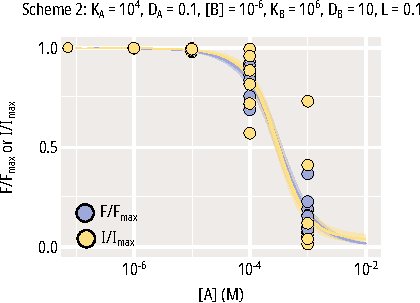
\includegraphics[width=\textwidth]{mwc_scheme_2_kb_shift.pdf}
	\end{subfigure}
	\hfill
	\begin{subfigure}[t]{0.45\textwidth}
		\caption{}\label{ch4fig:scheme_3_kb_shift}
		\centering
		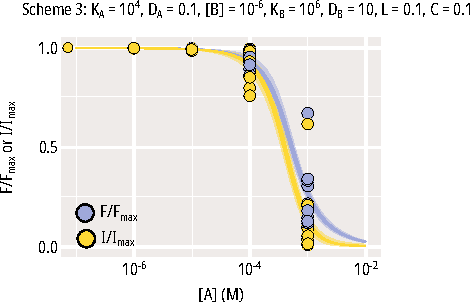
\includegraphics[width=\textwidth]{mwc_scheme_3_kb_shift.pdf}
	\end{subfigure}
	\vfill
	\begin{subfigure}[t]{0.9\textwidth}
		\caption{}\label{ch4fig:mwc_params_3}
		\centering
		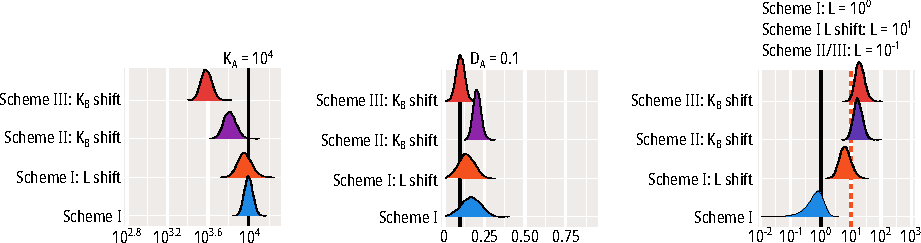
\includegraphics[width=\textwidth]{mwc_scheme_param_fits_3.pdf}
	\end{subfigure}
	\caption[Parameter retrieval from MWC models]{
	\subref{ch4fig:scheme_2_kb_shift}, \subref{ch4fig:scheme_3_kb_shift} Data generated from \subref{ch4fig:scheme_2_kb_shift} Scheme II  or \subref{ch4fig:scheme_3_kb_shift} with $K_B$ shifted from $10^5$ to $10^6$.
	}\label{ch4fig:scheme_2_3_shifts}
\end{figure}

However, it is unclear how changes in parameters which are not explicitly modelled in Scheme I will affect the generated data and the parameter estimates obtained by fitting the data to Scheme I.
Figure \ref{ch4fig:scheme_2_3_shifts} shows the results of increasing $K_B$ by tenfold on data generated from Scheme II (Figure \ref{ch4fig:scheme_2_kb_shift}) or Scheme III (Figure \ref{ch4fig:scheme_3_kb_shift}).
The first observation of note is that the generated data closely resemble those generated from Scheme I when $L$ is increased (Figure \ref{ch4fig:scheme_1_l_shift}), and indeed when the $L$ parameter estimates for a tenfold shift in $K_B$ in Scheme II/III and tenfold shift in $L$ for Scheme I are compared (Figure \ref{ch4fig:mwc_params_3}, right panel) are compared they appear to be similar.
So far so good, as an observed increase in $L$ when fit with Scheme I would lead us to draw the correct inferences about changes in the underlying model (i.e. the open probability of the cnall has indeed increased).
However, changes in $K_B$ are not perfectly captured by changes in $L$ when fit to scheme I.
Notably, if local allostery exists between the nucleotide and PIP\textsubscript{2} binding site - if Scheme III is the true underlying model - then fitting the observed data to Scheme I would lead us to estimate an incorrect value for $K_A$ (Figure \ref{ch4fig:scheme_2_kb_shift}).
Thus, if there is local allostery between the sites, then a mutation which induces an increase in the binding affinity for PIP\textsubscript{2} would not just increase our estimate of $L$ (which would lead to a correct inference) but it would also decrease our estimate of $K_A$ by a not-insignificant amount, which could lead to the incorrect inference that a mutation is causing a direct change in nucleotide binding when it is in fact causing a direct change in PIP\textsubscript{2} binding, which through local allostery is influencing our estimates of $K_A$.
